
%%%%%%%%%%%%%%%%%%%%%%%%%%%%%%%%%%%%%%%%%%%%%%
\section{Installation}


%%%%%%%%%%%%%%%%%%%%%%
\subsection{Anode Plane Assemblies (APAs)}

The APAs will be delivered to EHN1 in containers as shipped from the production sites.  These containers will be opened inside EHN1 and special lifting fixtures will be attached to each end of the APA.  The APA will be positioned and attached to the two conveyances in EHN1.  Both conveyances will used to lift the APA from the container and then rotate 90° from the orientation from which it was shipped.  The lifting strap and fixtures will be removed for the lower edge of the APA.  This orientation of the APA is shown in Figure~\ref{APA-tooling}.

\begin{cdrfigure}[The APA with the special tooling attached]{APA-tooling}{The APA with the lifting tooling attached.  The right image shows the orientation of the APA as delivered, the left shows the orientation when it is lowered into the material SAS. }
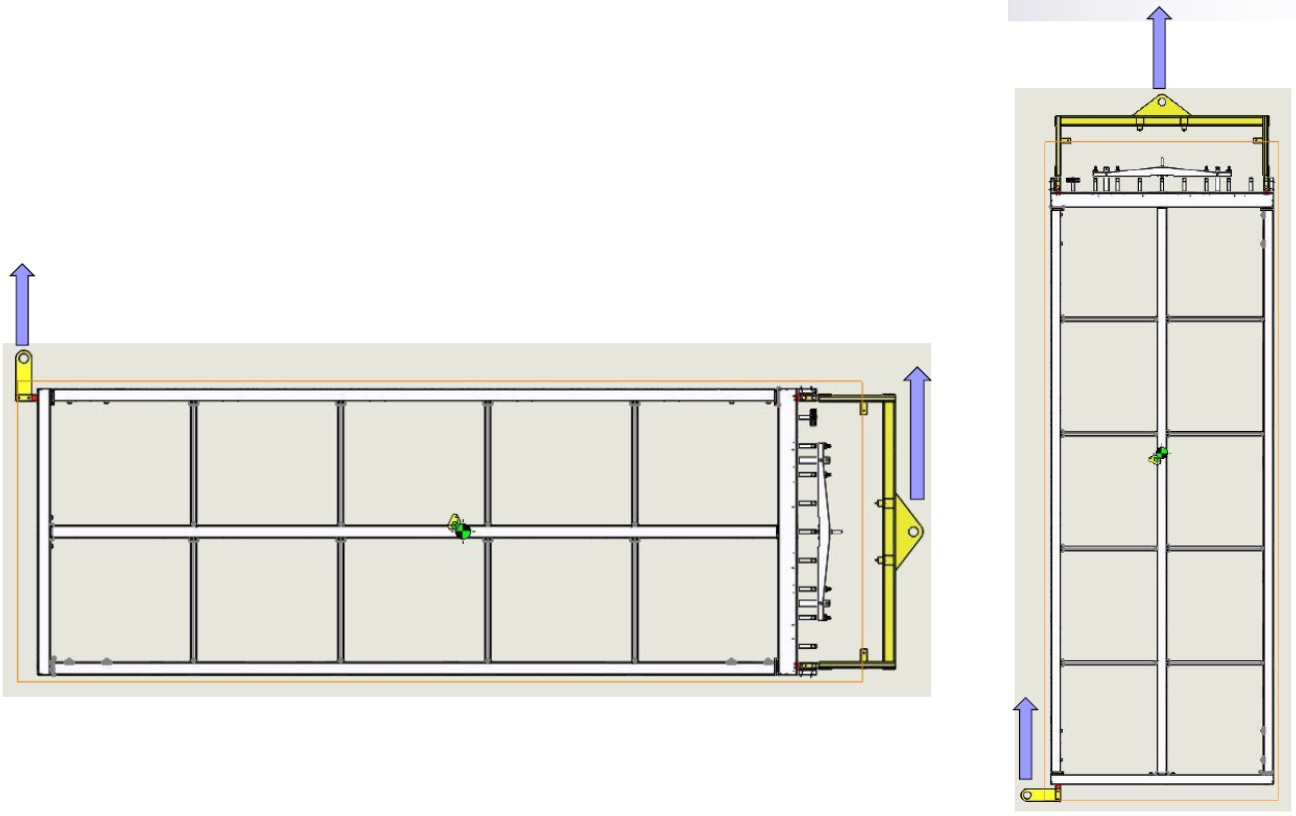
\includegraphics[width=1.00\linewidth]{apa-tooling}
\end{cdrfigure}

Once the APA is removed from the container and properly oriented, the roof hatch on the material SAS for the clean room will be opened and the APA will be lowered down through.  The APA will then be transferred to a rolling trolley attached to the series of rails in the cleanroom.  These rails are described in more detail in section 6.1.  It will be moved into the cleanroom via these rails.  

The APA will then go through a series of acceptance tests.  These tests include both electrical and wire tension.  It will also be inspected for broken wires or any other damage that could have resulted from shipment.  

After this testing is complete, the APA will be integrated with the PD system.  There are 10 PD per APA.  These are inserted into the sides of the APA frame.  This insertion alternates from one side to the other, with 5 PD being inserted into the APA from each direction.  This is shown in figure 4.122.  Once a PD is inserted, it is attached mechanically to the APA frame with fasteners and a single electronics cable is attached and strain relieved.  Each of the PD are tested immediately after installation to ensure proper operation and to verify the cable readout.  

The CE are installed on the APA once the PD installation is complete.  Each CE unit consists of an electronics enclosure that contains the TPC read-out electronics inside.  Each unit also includes a bundle of cables that connect the electronics to the outside of the cryostat via the flange on the feed through port.  Each APA will have 20 CE units installed at the top of the APA frame.  The location of the CE units on the APA is shown in Figure CE installation.  These units will be connected via matching electrical connectors on the FEMB and the CR board mounted on the APA.  There will also be mechanical fasteners to hold the enclosure to brackets supported by the APA frame.  Each of the CE units will be tested once installed to check connectivity.  

After the APA has been fully integrated with the PD and CE, it will be moved via the rails in the cleanroom to the integrated cold test stand.  This test stand, shown in Figure~\ref{cold-test-stand-open}, is a large insulated box that is light tight for PD testing and a Faraday shield for CE testing.  At the top of the box, there will be a crossing tube, similar to those in the cryostat, with a conflat fitting that will accept the warm – cold interface flange for the PD and CE cable connections.  The PD and CE cables will be routed and connected to their flanges, the APA will be moved inside and the end cover, that completes the Faraday cage, installed so that the integrated electronics testing can begin.  A series of warm tests will be performed.  This is described in XXsectionXX.  \fixme{}
After the warm tests are complete, the inner volume of the enclosure will be purged with dry gas to reduce the moisture inside.  After this gas purge, the inner volume will be slowly cooled down using nitrogen gas to a temperature of approximately 100 $^\circ$K.  The rate of cooldown is to be less than 10 $^\circ$K/hr which is the same for the cryostat.  The cooldown system is being designed to maintain the inner volume near 100 $^\circ$K for approximately 48 hours.  The cold testing of the can be performed during the cooldown period, during these 48 hr and during the warmup.  After the testing is complete and the box has been purged of nitrogen with room air, it will be opened, the APA removed and he cables disconnected and secured for movement on the rail system.   

\begin{cdrfigure}[Cold test stand]{cold-test-stand-open}{Cold test stand }
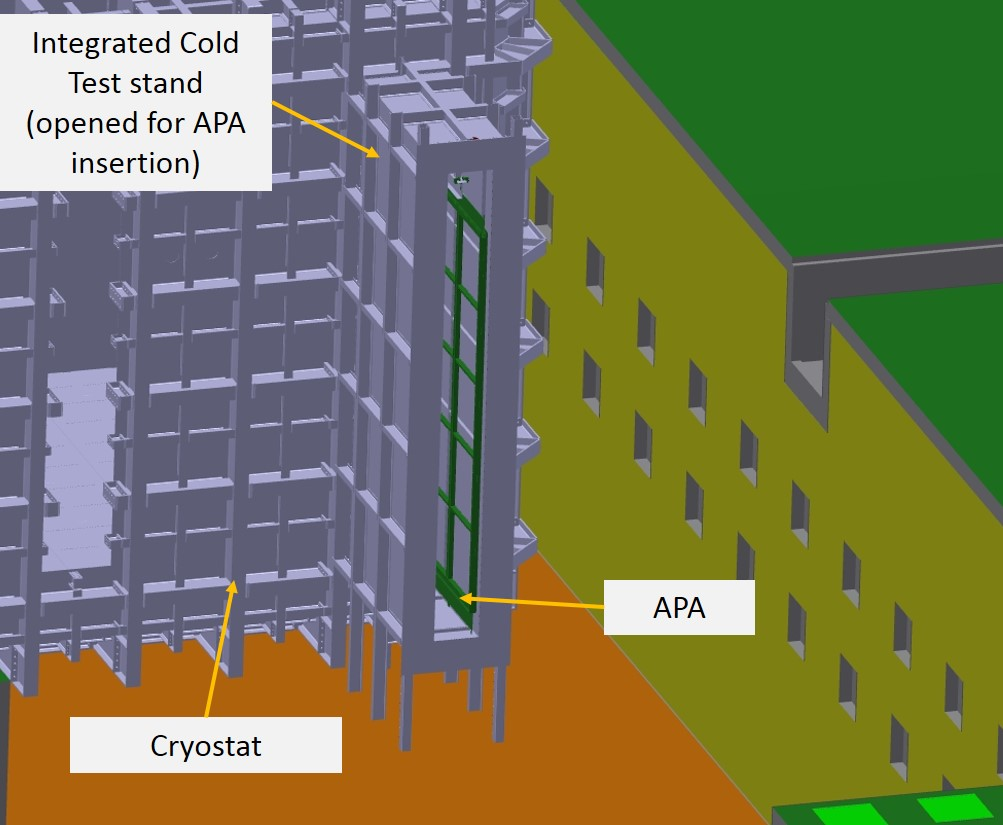
\includegraphics[width=1.00\linewidth]{cold-test-stand-open}
\end{cdrfigure}

\fixme{got this figure from jack; was titled 2016-09-08-Section4.9.9\_Figure\_4.cold test stand}

The APA is now ready to be moved into the cryostat.  This will be done via the rail system in the clean room.  The APA will be moved through the TCO and transferred onto the appropriate rail in the detector support system.  Inside the cryostat, three APAs are needed to complete one row for the TPC.  When the next two APAs are delivered, integrated and tested, they will be moved onto the same rail.  The mechanical linkages between the APA will be installed and the trio will be surveyed and locked into position in the beam direction.  Once positioned, the entire rail with the three APAs will be translated in into position in the Y direction.  The cables from each of the CE and PDs on the APA will be routed and connected to the final flanges on the cryostat.  

At the appropriate time in the installation sequence, the second trio of APAs will be moved into the cryostat and onto their detector support rail.  They will be surveyed and positioned in the same manner.


%%%%%%%%%%%%%%%%%%%%%%
\subsection{Cathode Plane Assemblies (CPAs)}

%\subsection{Assembly  and Installation }

\fixme{Jack will revise this} 

Individual CPA panels will be assembled off site and shipped to CERN in the horizontal position.  Each panel weights roughly 24 kgs and therefore can be lifted out of the shipping crate by hand and will not require and special fixtures.

The three CPA modules that make up a CPA panel will be placed on a flat surface and screwed/pinned together.   The crane then will be attached at the top end of the CPA with appropriate lifing straps and shackles.  The assembled CPA panel will be lifted to the vertical position.  

The load transfer from the crane hook to the installation rail still needs to be determined.  

Once two CPA planes are mounted they must be brought together within 1mm along their length.  (see thermal discussion in Section 7).  There will be two pins located on the side of the first CPA that will have to fit into a vertical slot on the side of the second CPA to lock them together in plane.  

The CPA plane may not hang vertically after being hung if the strap is not perfectly on center.  This can be corrected when the FC are mounted to a pair of CPA planes.  The connection points on the FC is fixed and therefore will tie the CPA’s together and force them to hang vertically because the assembly of the CPA planes and FC then becomes a two point support structure.  

During assembly the FC will be hung from the CPA.  In a worst case scenario the two FC will be mounted on one side of the CPA first which will cause the CPA to rotate 2.9'' due to the offset loading.  



%%%%%%%%%%%%%%%%%%%%%%
\subsection{Field Cage (FC)}

%\subsection{Assembly Sequence and QC Procedures}

There are three basic elements that comprise the FC for the TPC.  They are the top FC assembly, bottom FC assembly and the end wall FC assembly.  The top and bottom FC assemblies are basically mirror assemblies that will be hinged from the top and bottom of the CPA modules.  Figure~\ref{FC-assy} (left) shows a top/bottom FC assembly.  The ground plane covers one side of the field shaping profiles.  Figure~\ref{FC-assy} (right) shows a top and bottom FC attached only to one side of the CPA module.  These will be attached to both sides for the ProtoDUNE installation.  

\begin{cdrfigure}[Top/bottom FC assembly]{FC-assy}{Top/bottom FC assembly }
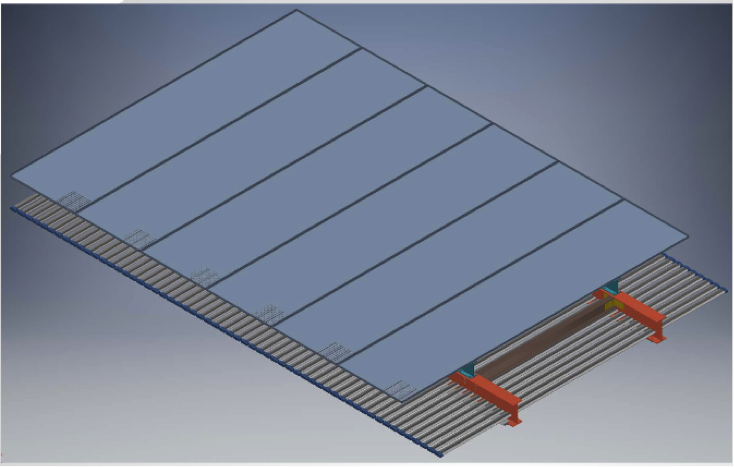
\includegraphics[width=.80\linewidth]{top-bottom-fc-assembly}
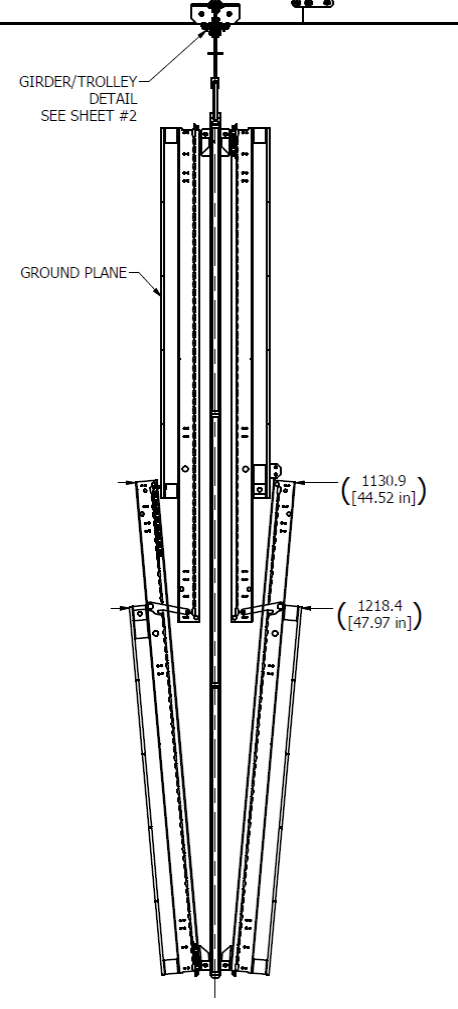
\includegraphics[width=0.1\linewidth]{fc-assy-vertical}
\end{cdrfigure}

The end wall FC are constructed from end wall FC modules.  Figure~\ref{FC-end-wall-panel} shows one of the end wall FC modules.  Four of these modules will be stacked and connected together to build the end wall.  This will be done by the overhead hoist near the TCO in the clean room.  Once the end wall is complete, it will be moved into the cryostat on the rails in the clean room and positioned on the appropriate beam in the DSS.  The end wall will be support by a spreader bar supported from the beam and have the ability to swivel about the support point.  This is necessary for positioning the end wall with respect to the APA and CPA in the installation process.  

\begin{cdrfigure}[FC end wall panel]{FC-end-wall-panel}{FC end wall panel }
%\includegraphics[width=.80\linewidth]{}
\end{cdrfigure}
\fixme{Jack needs to remake the fc end wall panel picture}

The sequence of installation for the FC components is as follows:
\begin{itemize}
\item After the first row of APAs is installed and translated to the Saleve side of the cryostat, the two end walls for the Saleve drift will be constructed and moved inside the cryostat supported by X beam B.  
\item As the CPA modules are constructed outside the cryostat, both the top and bottom FC assemblies will be attached on both sides top and bottom.  This combination of FC and CPA will then be moved into the cryostat and supported by X beam C.  This will be completed three times to get all into postion.
\item After the second row of APAs is installed and translated to the Jura side of the cryostat, the two end walls for the Jura drift will be constructed and moved inside the cryostat supported by X beam D.  
\end{itemize}


%%%%%%%%%%%%%%%%%%%%%%
\subsection{Photon Detection System (PDS)}

\fixme{no text here; got this figure from Jack, it was titled 2016-09-08-Section4.9.9\_Figure\_4.PD install, or something like that. Anne}

\begin{cdrfigure}[PDS installation]{pds-install}{PDS installation}
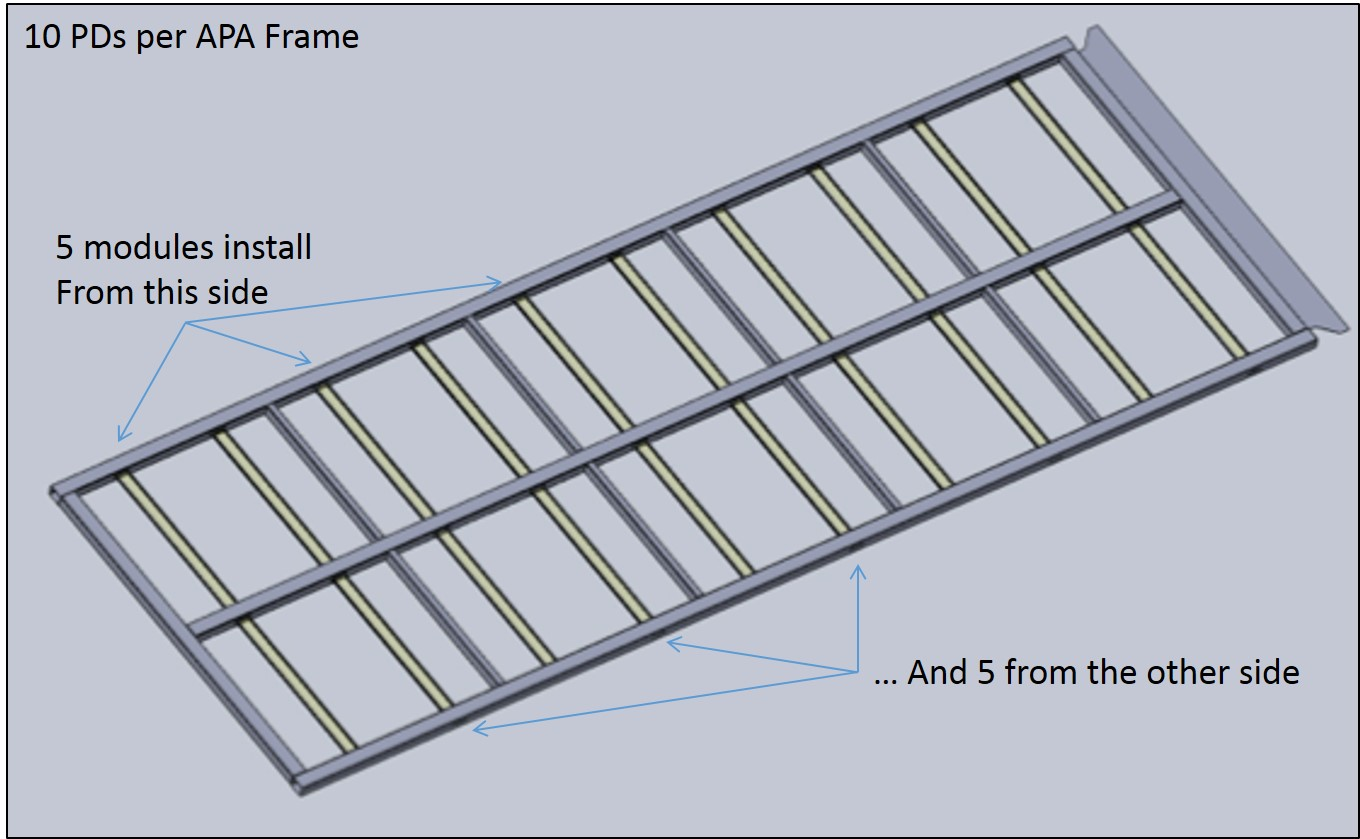
\includegraphics[width=1.00\linewidth]{pds-installation}
\end{cdrfigure}



%%%%%%%%%%%%%%%%%%%%%%
\subsection{Cold Electronics (CE)}
\label{subsec:ce_install}

Cold electronics will be mounted on the TPC and installed inside the cryostat.
Because access to the cold electronics is not possible after the cryostat is sealed,
a full complement of tests will be performed during the development stage and before the final installation
(Figure~\ref{fig:tpcce_CMBonAPA}).

\begin{cdrfigure}[The front end electronics as mounted on an APA]{tpcce_CMBonAPA}{The front end electronics as mounted on an APA.
  {\bf Top:} The front end electronics  is shown in the red circle.
  {\bf Bottom:} Cross section view.}
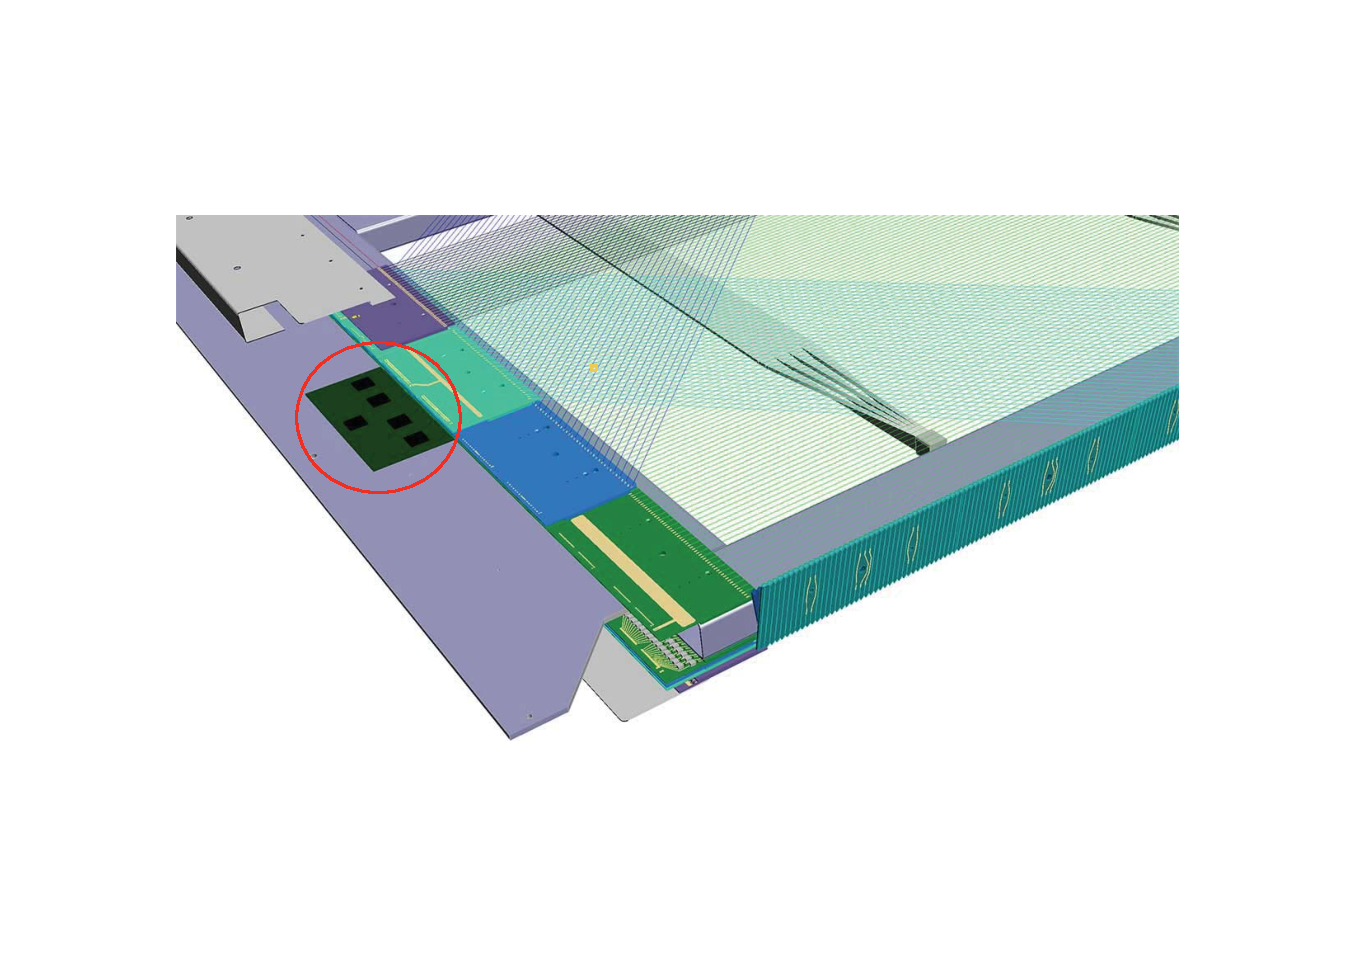
\includegraphics[width=1.00\linewidth]{tpcce_CMBonAPA_1.pdf}
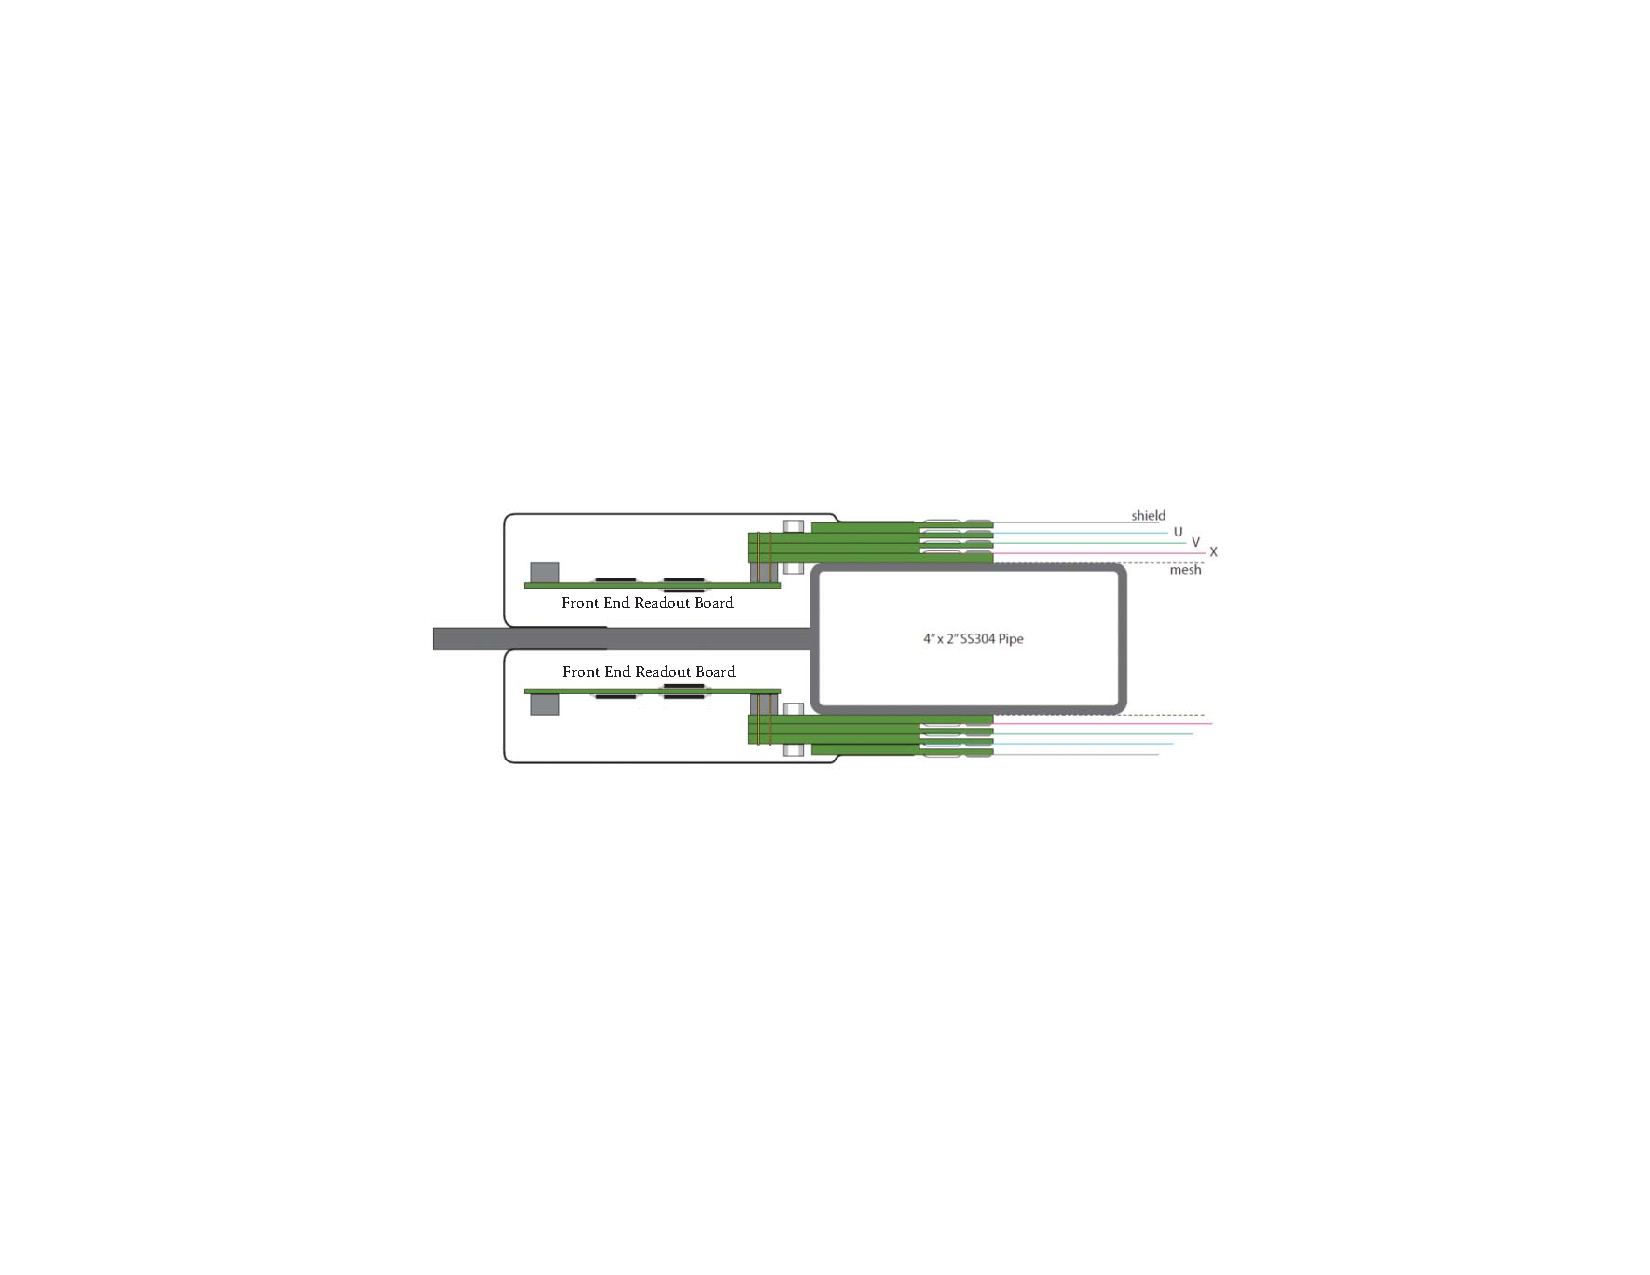
\includegraphics[width=1.00\linewidth]{tpcce_CMBonAPA_2.pdf}
\end{cdrfigure}

\fixme{Have two instances of this figure; we'll need to get rid of one. Anne}

\fixme{next figure: got from jack; titled 2016-09-08-Section4.9.9\_Figure\_4.CE installation.jpg. Does it go here?}

\begin{cdrfigure}[CE installation]{ce-install}{CE installation}
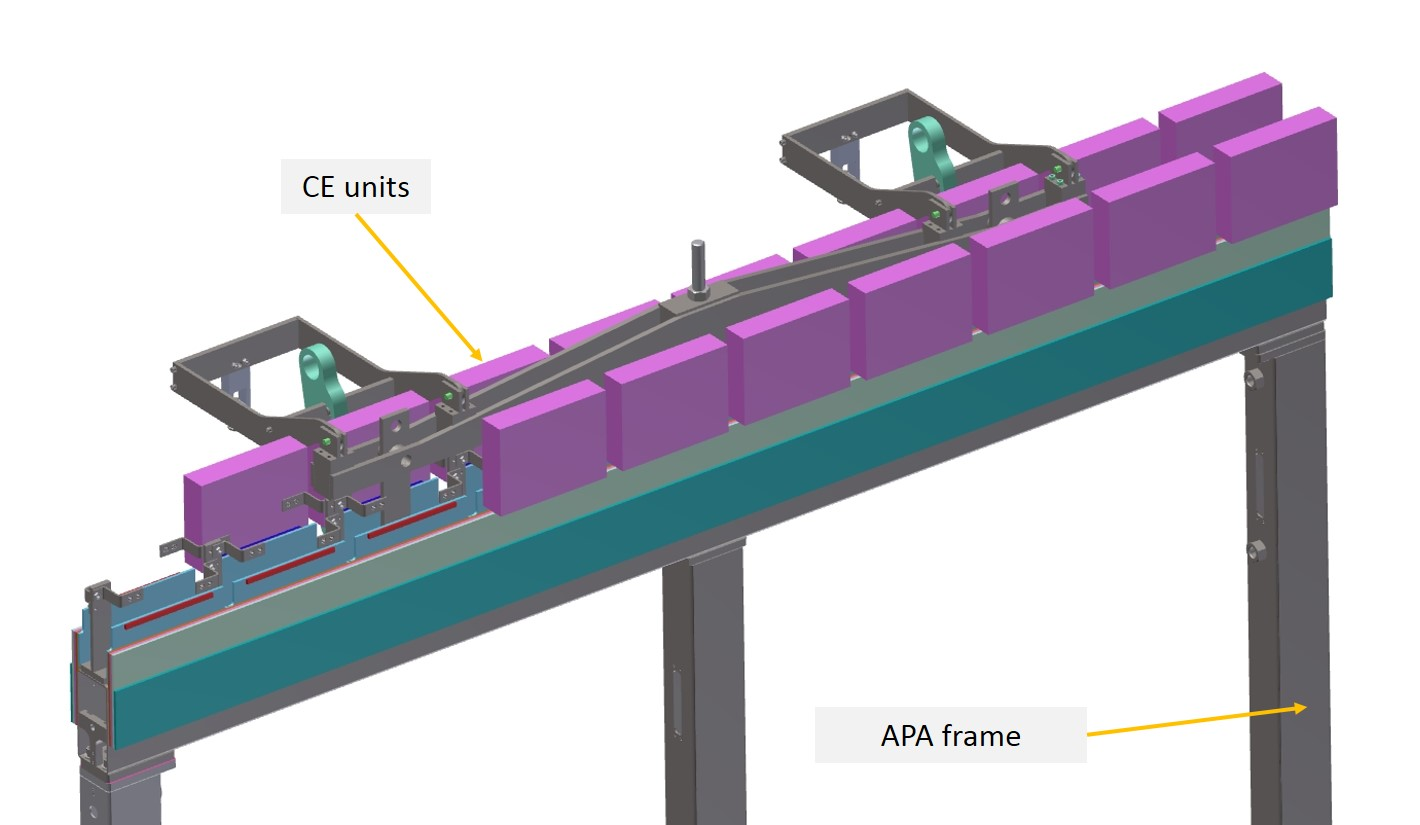
\includegraphics[width=1.00\linewidth]{ce-installation}
\end{cdrfigure}


%%%%%%%%%%%%%%%%%%%%%%%%%
\subsection{QC Procedures}

